\documentclass[10pt,a4paper]{article}

\usepackage{amsmath}
\usepackage{amsfonts}
\usepackage{amssymb}
\usepackage{graphicx}
\usepackage{multicol}
\usepackage{tabularx}
\usepackage{tikz}
\usetikzlibrary{arrows,shapes,automata,petri,positioning,calc}
\usepackage{hyperref}
\usepackage{tikz}
\usetikzlibrary{matrix,calc}
\usepackage[margin=0.5in]{geometry}
\newcommand{\myvec}[1]{\ensuremath{\begin{pmatrix}#1\end{pmatrix}}}
\let\vec\mathbf
\newenvironment{Figure}
  {\par\medskip\noindent\minipage{\linewidth}}
  {\endminipage\par\medskip}
\begin{document}
%--------------------logo figure-------------------------%
\begin{figure*}[!tbp]
 \centering
  \begin{minipage}[b]{0.4\textwidth}
  
\includegraphics[scale=.25]{iitlogo.png} 
  \end{minipage}
\end{figure*}
%--------------------name & rollno-----------------------
\raggedright \textbf{Name}:\hspace{1mm} Ganga Gopinath\hspace{3cm} \Large \textbf{Matrix Assignment}\hspace{2.5cm} % 
\normalsize \textbf{Roll No.} :\hspace{1mm} FWC22050\vspace{1cm}
\begin{multicols}{2}
\section{Problem statement:}  Construct a triangle PQR in which QR=6cm, $\angle{Q}=60^0$ and PR - PQ = 2cm.\vspace{3mm}


\textbf{Law of Cosines}
\vspace{2mm}\raggedright \\

The law of Cosines relates the length of the triangle to the cosines of one of its angles. It states that, if the length of two sides and the angle between them is known for a triangle, then we can determine the length of the third side. It is given by:
\begin{equation}
\vec{b}^2=\vec{a}^2+\vec{c}^2-2accosB 
 \end{equation}

%-----------------------------solution---------------------------
\raggedright \textbf{SOLUTION}:\vspace{2mm}\\
\raggedright \textbf{Steps of Construction:}\\

1.Draw a line segment of base QR = 6 cm

2. Measure and draw  $\angle{Q}=60^0$ and let the ray be QX

3. Using a compass measure PR-PQ = 2cm.

4. As PQ-PR is negative, QD will below the line QR.

5. With Q as a centre and draw an arc with radius 2cm at the point be D on the ray QX

6. Join DR

7. Draw the perpendicular bisector of the line DR and the intersection point is taken as P.

8. Join PR

9. PQR is the required triangle.

\vspace{5mm}
\textbf{By Law of Cosines :} \vspace{3mm}


\textbf{To Construct}\vspace{2mm}\\
Let P,Q and R be the vertices of the triangle  with coordinates.

\raggedright\textbf{STEP-1}\vspace{2mm}\\

Then coordinates of vertices  Q,R and P are :\vspace{2mm}\\
\begin{center}$
\vec{
 Q =\begin{pmatrix}
0 \\
0 
\end{pmatrix} 
\vspace{1mm}
R=\begin{pmatrix}
6 \\
0 
\end{pmatrix} 
\vspace{1mm}
P=r\begin{pmatrix}
sin \theta\\
  cos \theta\\
\end{pmatrix} }
\vspace{1mm}$
\end{center}

\vspace{3mm} 
By using the Cosine formula in  $\Delta$PQR \\ 
\begin{equation}
\vec{q}^2=\vec{p}^2+\vec{r}^2-2prcosB 
\end{equation}
\begin{center}
$0=\vec{p}^2+\vec{r}^2 -\vec{q}^2-2prcosQ 
\vspace{5mm}
\newline
$0=(r+q)(r-q)+${6}^2$ - 2 $\times$ 6 $\times$ .5r\\
\vspace{5mm}
\end{center}
After simplification
\begin{equation}
   2r-q =18
\end{equation}
Given that,
\begin{equation}
r-q=2
\end{equation}


Using equation (3) and (4),
\begin{equation}
  \begin{pmatrix}
2 & -1\\
1 &-1
\end{pmatrix} 
\begin{pmatrix}
r\\
q
\end{pmatrix} 
=
\begin{pmatrix}
18 \\
 2\
\end{pmatrix}
\end{equation}\vspace{2mm}\\

 Let,
\begin{equation}
\vec{A} =\begin{pmatrix}
2 & -1\\
1 &-1
\end{pmatrix} 
\end{equation} \\ \vspace{2mm}
\begin{equation}
  \vec{X} =\begin{pmatrix}
r \\
y
\end{pmatrix} 
\end{equation}  \vspace{2mm}

\begin{equation}
 \vec{B} = \begin{pmatrix}
18\\
2
\end{pmatrix} 
\end{equation} \vspace{2mm}
We know that,\\
\begin{equation}
\vec{A  X = B}
\end{equation}
And,\\
\begin{equation}
\vec{A^{-1} A = I}
\end{equation}
multiplying $A^{-1}$ on both sides in equation (9)\\
\begin{equation}
 \vec{X = A^{-1} B}
\end{equation}
Using equation (11) we get ,
\begin{equation}
r = 16 \vspace{2mm}
\end{equation}
\begin{equation}
 q = 14 \vspace{2mm}
\end{equation}
The vertices of $\Delta$ PQR are \\
\begin{equation}
P= 16 \begin{pmatrix}
cos 45\\
sin 45\\
\end{pmatrix} 
,Q= \begin{pmatrix}
 0\\
 0\\
 \end{pmatrix} 
,R= \begin{pmatrix}
 6\\
 0\\
\end{pmatrix} 
\end{equation} \vspace{2mm}


\textbf{Result} 
\begin{center}
 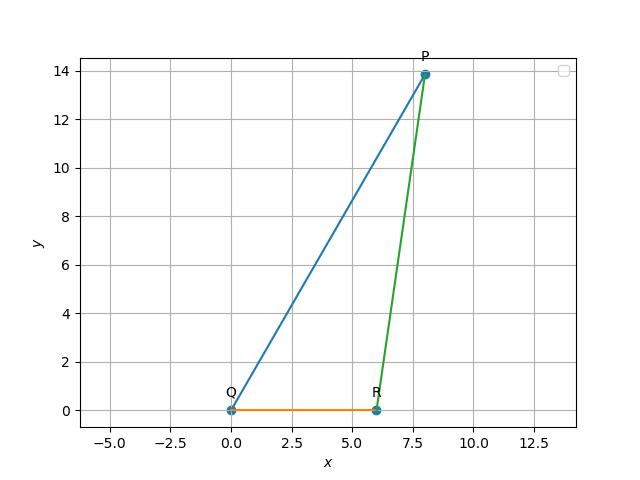
\includegraphics[width=0.4\textwidth]{ex2.jpg}  
 \end{center}\vspace{5mm}
 \vspace{2mm}  
\textbf{Implementation}
\begin{center}
\setlength{\arrayrulewidth}{0.5mm}
\setlength{\tabcolsep}{5pt}
\renewcommand{\arraystretch}{3}
    \begin{tabular}{|l|c|}
    \hline 
    \textbf{Equation no} & \textbf{Role} \\ \hline
    1 &  law of Cosines \\ 
    5 & Matrix form of Linear equation  \\
    10 & Results Identity matrix  \\
    12 & Length of r\\
    13 & Length of q \\
    
    \hline
      \end{tabular}
  \end{center} \vspace{2mm}
  
 
\raggedright  Download the code \\
https://github.com/Gangagopinath/ASSIGNMENT/tree/
\newline
main/assignment4
  \end{multicols}
\end{document}